% Sketch output, version 0.3 (build 2d, Wed Apr 20 23:38:45 2011)
% Output language: PGF/TikZ,LaTeX
\documentclass[letterpaper,12pt]{article}
\usepackage[x11names,rgb]{xcolor}
\usepackage{tikz}
\usetikzlibrary{snakes}
\usetikzlibrary{arrows}
\usetikzlibrary{shapes}
\usetikzlibrary{backgrounds}
\usepackage{amsmath}
\oddsidemargin 0in
\evensidemargin 0in
\topmargin 0in
\headheight 0in
\headsep 0in
\textheight 9in
\textwidth 6.5in
\begin{document}
\pagestyle{empty}
\vspace*{\fill}
\begin{center}
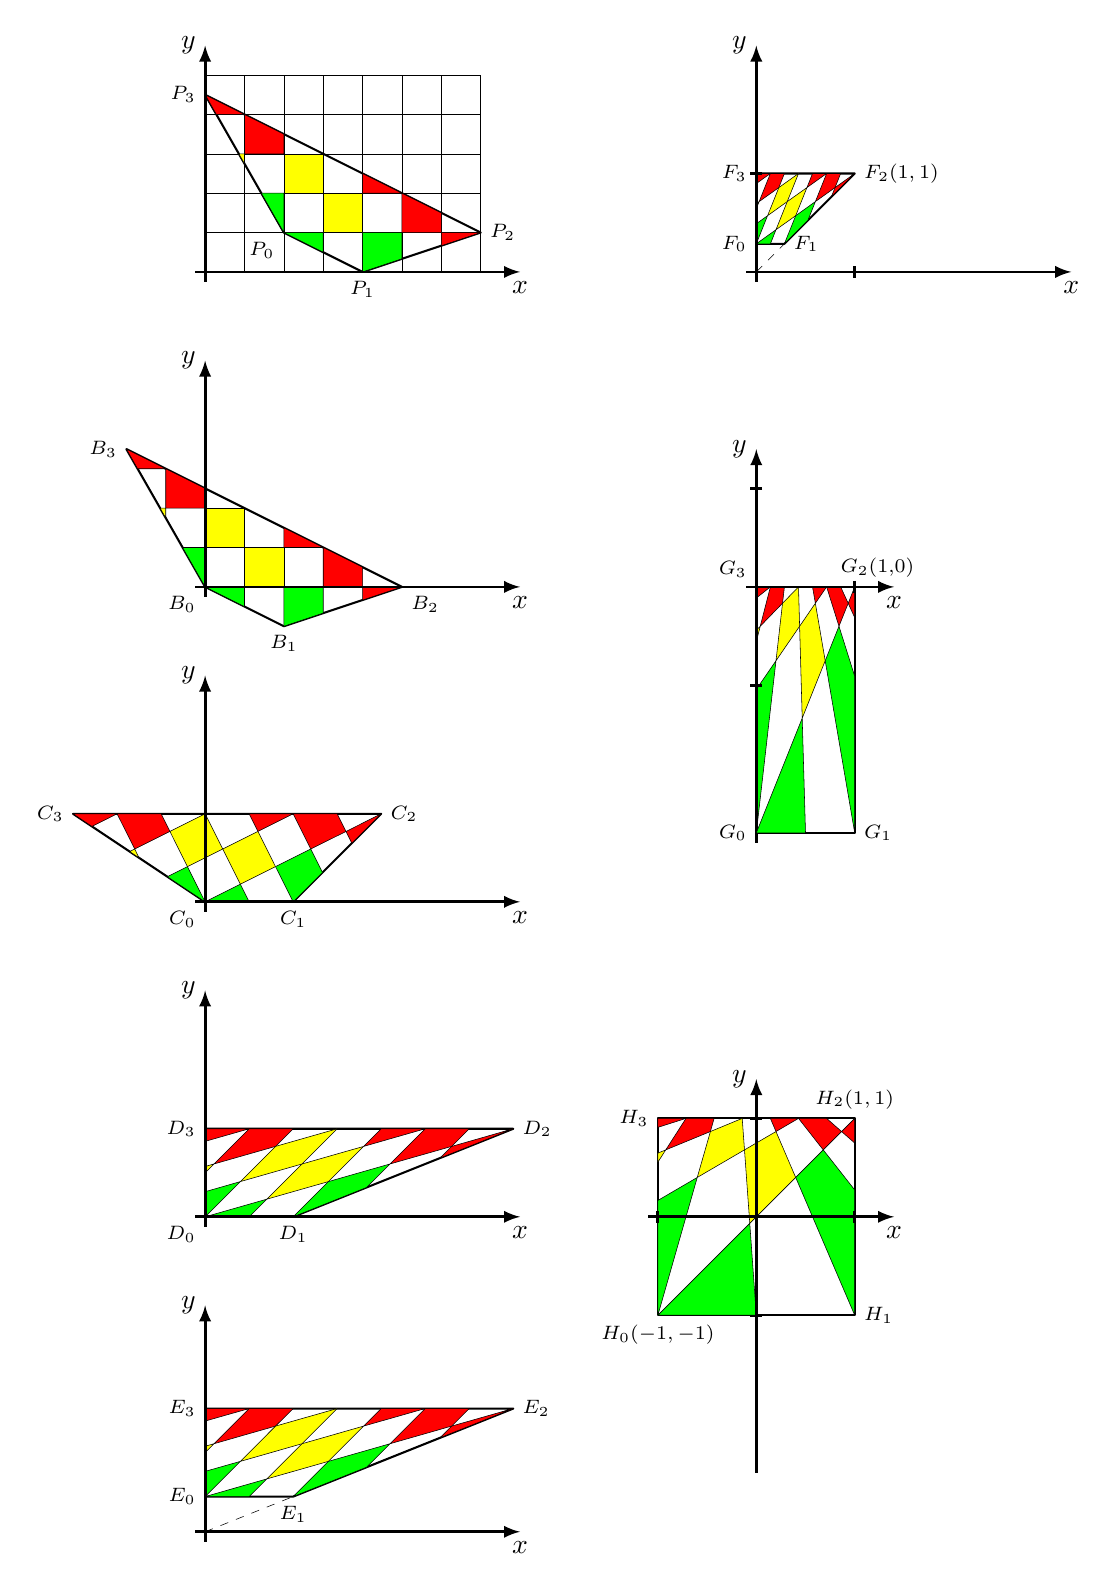
\begin{tikzpicture}[line join=round,line width=0.2pt,>=latex]
\filldraw[fill=none,line width=0.75pt](1,.5)--(2,0)--(3.5,.5)--(0,2.25)--cycle;
\filldraw[fill=none,line width=0.75pt](7,-7.125)--(8.25,-7.125)--(8.25,-4)--(7,-4)--cycle;
\draw[dashed](7,0)--(7.357,.357);
\filldraw[fill=none,line width=0.75pt](7,.357)--(7.357,.357)--(8.25,1.25)--(7,1.25)--cycle;
\draw[dashed](0,-16)--(1.118,-15.553);
\filldraw[fill=none,line width=0.75pt](0,-15.553)--(1.118,-15.553)--(3.913,-14.435)--(0,-14.435)--cycle;
\filldraw[fill=none,line width=0.75pt](0,-12)--(1.118,-12)--(3.913,-10.882)--(0,-10.882)--cycle;
\filldraw[fill=none,line width=0.75pt](0,-8)--(1.118,-8)--(2.236,-6.882)--(-1.677,-6.882)--cycle;
\filldraw[fill=none,line width=0.75pt](0,-4)--(1,-4.5)--(2.5,-4)--(-1,-2.25)--cycle;
\draw(0,2.5)--(3.5,2.5);
\draw(0,2)--(3.5,2);
\draw(0,1.5)--(3.5,1.5);
\draw(0,1)--(3.5,1);
\draw(0,.5)--(3.5,.5);
\draw(0,0)--(3.5,0);
\draw(3.5,0)--(3.5,2.5);
\draw(3,0)--(3,2.5);
\draw(2.5,0)--(2.5,2.5);
\draw(2,0)--(2,2.5);
\draw(1.5,0)--(1.5,2.5);
\draw(1,0)--(1,2.5);
\draw(.5,0)--(.5,2.5);
\draw(0,0)--(0,2.5);
\filldraw[fill=red](3,.333)--(3.5,.5)--(3,.5)--cycle;
\filldraw[fill=red](2.5,.5)--(3,.5)--(3,.75)--(2.5,1)--cycle;
\filldraw[fill=red](2,1.25)--(2,1)--(2.5,1)--cycle;
\filldraw[fill=red](.5,2)--(.5,1.5)--(1,1.5)--(1,1.75)--cycle;
\filldraw[fill=red](0,2.25)--(.143,2)--(.5,2)--cycle;
\filldraw[fill=yellow](1.5,.5)--(2,.5)--(2,1)--(1.5,1)--cycle;
\filldraw[fill=yellow](1,1.5)--(1,1)--(1.5,1)--(1.5,1.5)--cycle;
\filldraw[fill=yellow](.5,1.5)--(.5,1.375)--(.429,1.5)--cycle;
\filldraw[fill=green](2,0)--(2.5,.167)--(2.5,.5)--(2,.5)--cycle;
\filldraw[fill=green](1,.5)--(1.5,.25)--(1.5,.5)--cycle;
\filldraw[fill=green](1,.5)--(1,1)--(.714,1)--cycle;
\filldraw[fill=none,line width=0.75pt](5.75,-13.25)--(8.25,-13.25)--(8.25,-10.75)--(5.75,-10.75)--cycle;
\filldraw[fill=yellow](6.417,-10.917)--(6.25,-11.5)--(6.85,-11.15)--(6.821,-10.75)--cycle;
\filldraw[fill=red](8.25,-4.391)--(8.25,-4)--(8.167,-4.208)--cycle;
\filldraw[fill=red](8.05,-4.5)--(8.167,-4.208)--(8.071,-4)--(7.893,-4)--cycle;
\filldraw[fill=red](7.714,-4)--(7.75,-4.208)--(7.893,-4)--cycle;
\filldraw[fill=red](7.179,-4)--(7.05,-4.5)--(7.333,-4.208)--(7.357,-4)--cycle;
\filldraw[fill=red](7,-4)--(7,-4.142)--(7.179,-4)--cycle;
\filldraw[fill=yellow](7.333,-4.208)--(7.25,-4.938)--(7.55,-4.5)--(7.536,-4)--cycle;
\filldraw[fill=red](5.75,-10.75)--(5.75,-10.864)--(6.107,-10.75)--cycle;
\filldraw[fill=red](6.107,-10.75)--(5.85,-11.15)--(6.417,-10.917)--(6.464,-10.75)--cycle;
\filldraw[fill=red](8.25,-11.063)--(8.25,-10.75)--(8.083,-10.917)--cycle;
\filldraw[fill=red](7.85,-11.15)--(8.083,-10.917)--(7.893,-10.75)--(7.536,-10.75)--cycle;
\filldraw[fill=red](7.179,-10.75)--(7.25,-10.917)--(7.536,-10.75)--cycle;
\filldraw[fill=red](7.952,.952)--(8.25,1.25)--(8,1.071)--cycle;
\filldraw[fill=red](7.75,.893)--(8,1.071)--(8.071,1.25)--(7.893,1.25)--cycle;
\filldraw[fill=red](7.714,1.25)--(7.643,1.071)--(7.893,1.25)--cycle;
\filldraw[fill=red](7.179,1.25)--(7.036,.893)--(7.286,1.071)--(7.357,1.25)--cycle;
\filldraw[fill=red](7,1.25)--(7,1.122)--(7.179,1.25)--cycle;
\filldraw[fill=yellow](7.25,.536)--(7.5,.714)--(7.643,1.071)--(7.393,.893)--cycle;
\filldraw[fill=yellow](7.286,1.071)--(7.143,.714)--(7.393,.893)--(7.536,1.25)--cycle;
\filldraw[fill=yellow](7.036,.893)--(7,.804)--(7,.867)--cycle;
\filldraw[fill=green](7.357,.357)--(7.655,.655)--(7.75,.893)--(7.5,.714)--cycle;
\filldraw[fill=green](7,.357)--(7.179,.357)--(7.25,.536)--cycle;
\filldraw[fill=green](7,.357)--(7.143,.714)--(7,.612)--cycle;
\filldraw[fill=red](2.981,-14.807)--(3.913,-14.435)--(3.13,-14.658)--cycle;
\filldraw[fill=red](2.348,-14.882)--(3.13,-14.658)--(3.354,-14.435)--(2.795,-14.435)--cycle;
\filldraw[fill=red](2.236,-14.435)--(2.012,-14.658)--(2.795,-14.435)--cycle;
\filldraw[fill=red](.559,-14.435)--(.112,-14.882)--(.894,-14.658)--(1.118,-14.435)--cycle;
\filldraw[fill=red](0,-14.435)--(0,-14.594)--(.559,-14.435)--cycle;
\filldraw[fill=yellow](.783,-15.329)--(1.565,-15.106)--(2.012,-14.658)--(1.23,-14.882)--cycle;
\filldraw[fill=yellow](.894,-14.658)--(.447,-15.106)--(1.23,-14.882)--(1.677,-14.435)--cycle;
\filldraw[fill=yellow](.112,-14.882)--(0,-14.994)--(0,-14.914)--cycle;
\filldraw[fill=green](1.118,-15.553)--(2.05,-15.18)--(2.348,-14.882)--(1.565,-15.106)--cycle;
\filldraw[fill=green](0,-15.553)--(.559,-15.553)--(.783,-15.329)--cycle;
\filldraw[fill=green](0,-15.553)--(.447,-15.106)--(0,-15.233)--cycle;
\filldraw[fill=red](2.981,-11.255)--(3.913,-10.882)--(3.13,-11.106)--cycle;
\filldraw[fill=red](2.348,-11.329)--(3.13,-11.106)--(3.354,-10.882)--(2.795,-10.882)--cycle;
\filldraw[fill=red](2.236,-10.882)--(2.012,-11.106)--(2.795,-10.882)--cycle;
\filldraw[fill=red](.559,-10.882)--(.112,-11.329)--(.894,-11.106)--(1.118,-10.882)--cycle;
\filldraw[fill=red](0,-10.882)--(0,-11.042)--(.559,-10.882)--cycle;
\filldraw[fill=yellow](.783,-11.776)--(1.565,-11.553)--(2.012,-11.106)--(1.23,-11.329)--cycle;
\filldraw[fill=yellow](.894,-11.106)--(.447,-11.553)--(1.23,-11.329)--(1.677,-10.882)--cycle;
\filldraw[fill=yellow](.112,-11.329)--(0,-11.441)--(0,-11.361)--cycle;
\filldraw[fill=green](1.118,-12)--(2.05,-11.627)--(2.348,-11.329)--(1.565,-11.553)--cycle;
\filldraw[fill=green](0,-12)--(.559,-12)--(.783,-11.776)--cycle;
\filldraw[fill=green](0,-12)--(.447,-11.553)--(0,-11.681)--cycle;
\filldraw[fill=red](1.863,-7.255)--(2.236,-6.882)--(1.789,-7.106)--cycle;
\filldraw[fill=red](1.342,-7.329)--(1.789,-7.106)--(1.677,-6.882)--(1.118,-6.882)--cycle;
\filldraw[fill=red](.559,-6.882)--(.671,-7.106)--(1.118,-6.882)--cycle;
\filldraw[fill=red](-1.118,-6.882)--(-.894,-7.329)--(-.447,-7.106)--(-.559,-6.882)--cycle;
\filldraw[fill=red](-1.677,-6.882)--(-1.437,-7.042)--(-1.118,-6.882)--cycle;
\filldraw[fill=yellow](.447,-7.776)--(.894,-7.553)--(.671,-7.106)--(.224,-7.329)--cycle;
\filldraw[fill=yellow](-.447,-7.106)--(-.224,-7.553)--(.224,-7.329)--(0,-6.882)--cycle;
\filldraw[fill=yellow](-.894,-7.329)--(-.839,-7.441)--(-.958,-7.361)--cycle;
\filldraw[fill=green](1.118,-8)--(1.491,-7.627)--(1.342,-7.329)--(.894,-7.553)--cycle;
\filldraw[fill=green](0,-8)--(.559,-8)--(.447,-7.776)--cycle;
\filldraw[fill=green](0,-8)--(-.224,-7.553)--(-.479,-7.681)--cycle;
\filldraw[fill=red](2,-4.167)--(2.5,-4)--(2,-4)--cycle;
\filldraw[fill=red](1.5,-4)--(2,-4)--(2,-3.75)--(1.5,-3.5)--cycle;
\filldraw[fill=green](0,-4)--(0,-3.5)--(-.286,-3.5)--cycle;
\filldraw[fill=green](0,-4)--(.5,-4.25)--(.5,-4)--cycle;
\filldraw[fill=green](1,-4.5)--(1.5,-4.333)--(1.5,-4)--(1,-4)--cycle;
\filldraw[fill=yellow](-.5,-3)--(-.5,-3.125)--(-.571,-3)--cycle;
\filldraw[fill=yellow](0,-3)--(0,-3.5)--(.5,-3.5)--(.5,-3)--cycle;
\filldraw[fill=yellow](.5,-4)--(1,-4)--(1,-3.5)--(.5,-3.5)--cycle;
\filldraw[fill=red](-1,-2.25)--(-.857,-2.5)--(-.5,-2.5)--cycle;
\filldraw[fill=red](-.5,-2.5)--(-.5,-3)--(0,-3)--(0,-2.75)--cycle;
\filldraw[fill=red](1,-3.25)--(1,-3.5)--(1.5,-3.5)--cycle;
\filldraw[fill=yellow](7.583,-5.667)--(7.875,-4.938)--(7.75,-4.208)--(7.55,-4.5)--cycle;
\filldraw[fill=yellow](6.917,-12.083)--(7.5,-11.5)--(7.25,-10.917)--(6.85,-11.15)--cycle;
\filldraw[fill=yellow](7.05,-4.5)--(7,-4.694)--(7,-4.551)--cycle;
\filldraw[fill=green](8.25,-7.125)--(8.25,-5.136)--(8.05,-4.5)--(7.875,-4.938)--cycle;
\filldraw[fill=green](8.25,-13.25)--(8.25,-11.659)--(7.85,-11.15)--(7.5,-11.5)--cycle;
\filldraw[fill=yellow](5.85,-11.15)--(5.75,-11.306)--(5.75,-11.191)--cycle;
\filldraw[fill=green](5.75,-13.25)--(6.25,-11.5)--(5.75,-11.792)--cycle;
\filldraw[fill=green](7,-7.125)--(7.25,-4.938)--(7,-5.302)--cycle;
\draw[line width=1pt](7.075,-5.25)--(6.925,-5.25);
\draw[line width=1pt](7.075,-2.75)--(6.925,-2.75);
\draw[line width=1pt](8.25,-3.925)--(8.25,-4.075);
\draw[->,line width=1pt](7,-7.25)--(7,-2.25);
\draw[->,line width=1pt](6.875,-4)--(8.75,-4);
\draw[line width=1pt](7.075,1.25)--(6.925,1.25);
\draw[line width=1pt](8.25,.075)--(8.25,-.075);
\draw[->,line width=1pt](7,-.125)--(7,2.875);
\draw[->,line width=1pt](6.875,0)--(11,0);
\draw[->,line width=1pt](0,-16.125)--(0,-13.125);
\draw[->,line width=1pt](-.125,-16)--(4,-16);
\draw[->,line width=1pt](0,-12.125)--(0,-9.125);
\draw[->,line width=1pt](-.125,-12)--(4,-12);
\draw[->,line width=1pt](0,-8.125)--(0,-5.125);
\draw[->,line width=1pt](-.125,-8)--(4,-8);
\draw[->,line width=1pt](0,-4.125)--(0,-1.125);
\draw[->,line width=1pt](-.125,-4)--(4,-4);
\draw[->,line width=1pt](0,-.125)--(0,2.875);
\draw[->,line width=1pt](-.125,0)--(4,0);
\draw[line width=1pt](8.25,-11.925)--(8.25,-12.075);
\draw[line width=1pt](7.075,-10.75)--(6.925,-10.75);
\draw[line width=1pt](5.75,-11.925)--(5.75,-12.075);
\draw[line width=1pt](7.075,-13.25)--(6.925,-13.25);
\filldraw[fill=green](5.75,-13.25)--(7,-13.25)--(6.917,-12.083)--cycle;
\filldraw[fill=green](7,-7.125)--(7.625,-7.125)--(7.583,-5.667)--cycle;
\draw[->,line width=1pt](5.625,-12)--(8.75,-12);
\draw[->,line width=1pt](7,-15.25)--(7,-10.25);

    \coordinate [label=below:$x$] (X) at (4,0);
    \coordinate [label=left:$y$] (Y) at (0,2.875);
  
    \coordinate [label=225:\scriptsize$P_0$] (p0) at (1,.5);
    \coordinate [label=270:\scriptsize$P_1$] (p1) at (2,0);
    \coordinate [label=000:\scriptsize$P_2$] (p2) at (3.5,.5);
    \coordinate [label=180:\scriptsize$P_3$] (p3) at (0,2.25);
  
    \coordinate [label=below:$x$] (X) at (4,-4);
    \coordinate [label=left:$y$] (Y) at (0,-1.125);
  
    \coordinate [label=225:\scriptsize$B_0$] (p0B) at (0,-4);
    \coordinate [label=270:\scriptsize$B_1$] (p1B) at (1,-4.5);
    \coordinate [label=-60:\scriptsize$B_2$] (p2B) at (2.5,-4);
    \coordinate [label=180:\scriptsize$B_3$] (p3B) at (-1,-2.25);
  
    \coordinate [label=below:$x$] (X) at (4,-8);
    \coordinate [label=left:$y$] (Y) at (0,-5.125);
  
    \coordinate [label=225:\scriptsize$C_0$] (p0C) at (0,-8);
    \coordinate [label=270:\scriptsize$C_1$] (p1C) at (1.118,-8);
    \coordinate [label=000:\scriptsize$C_2$] (p2C) at (2.236,-6.882);
    \coordinate [label=180:\scriptsize$C_3$] (p3C) at (-1.677,-6.882);
  
    \coordinate [label=below:$x$] (X) at (4,-12);
    \coordinate [label=left:$y$] (Y) at (0,-9.125);
  
    \coordinate [label=225:\scriptsize$D_0$] (p0D) at (0,-12);
    \coordinate [label=270:\scriptsize$D_1$] (p1D) at (1.118,-12);
    \coordinate [label=000:\scriptsize$D_2$] (p2D) at (3.913,-10.882);
    \coordinate [label=180:\scriptsize$D_3$] (p3D) at (0,-10.882);
  
    \coordinate [label=below:$x$] (X) at (4,-16);
    \coordinate [label=left:$y$] (Y) at (0,-13.125);
  
    \coordinate [label=180:\scriptsize$E_0$] (p0E) at (0,-15.553);
    \coordinate [label=270:\scriptsize$E_1$] (p1E) at (1.118,-15.553);
    \coordinate [label=000:\scriptsize$E_2$] (p2E) at (3.913,-14.435);
    \coordinate [label=180:\scriptsize$E_3$] (p3E) at (0,-14.435);
  
    \coordinate [label=below:$x$] (X) at (11,0);
    \coordinate [label=left:$y$] (Y) at (7,2.875);
  
    \coordinate [label=180:\scriptsize$F_0$] (p0F) at (7,.357);
    \coordinate [label=000:\scriptsize$F_1$] (p1F) at (7.357,.357);
    \coordinate [label=000:{\scriptsize$F_2(1,1)$}] (p2F) at (8.25,1.25);
    \coordinate [label=180:\scriptsize$F_3$] (p3F) at (7,1.25);
  
    \coordinate [label=below:$x$] (X) at (8.75,-4);
    \coordinate [label=left:$y$] (Y) at (7,-2.25);
  
    \coordinate [label=180:\scriptsize$G_0$] (p0G) at (7,-7.125);
    \coordinate [label=  0:\scriptsize$G_1$] (p1G) at (8.25,-7.125);
    \coordinate [label= 90:{\scriptsize$G_2\makebox[0pt][l]{(1,0)}$}] (p2G) at (8.25,-4);
    \coordinate [label=135:\scriptsize$G_3$] (p3G) at (7,-4);
  
    \coordinate [label=below:$x$] (X) at (8.75,-12);
    \coordinate [label=left:$y$] (Y) at (7,-10.25);
  
    \coordinate [label=270:{\scriptsize$H_0(-1,-1)$}] (p0H) at (5.75,-13.25);
    \coordinate [label=  0:{\scriptsize$H_1$}]        (p1H) at (8.25,-13.25);
    \coordinate [label= 90:{\scriptsize$H_2(1,1)$}]   (p2H) at (8.25,-10.75);
    \coordinate [label=180:{\scriptsize$H_3$}]        (p3H) at (5.75,-10.75);
  \end{tikzpicture}
\end{center}
\vspace*{\fill}
\end{document}
% End sketch output
